\section{Modelos Matemáticos para Sistemas Continuos}

\begin{frame}{Ecuacion diferencial ordinaria en forma de espacio de estados explícita}
    \note{
    Existe una formulación estándar de las ecuaciones de ciertos modelos matemáticos de sistemas dinámicos denominada modelos de espacio de estados explícitos, en donde las derivadas de las variables de estado aparecen explícitamente del lado izquierdo de las ecuaciones.
    Estos modelos usualmente resultan más eficiente de resolver y analizar que otros modelos más complicados.\\
    El modelo expresado de esta manera implica que a partir de las variables de estado y de las variables de entrada podemos calcular las derivadas y las variables algebraicas. }
    \framesubtitle{Forma General}
    \begin{align*}
        \dot{x}(t) & =f(x(t),u(t)) \\
        y(t)       & =g(x(t),u(t))
    \end{align*}
\end{frame}

\begin{frame}{Ecuacion diferencial ordinaria en forma de espacio de estados explícita}
    \framesubtitle{Ejemplo: Ley de fuerza de Newton}   
    \begin{center}
        $m\ddot{s}(t)=F(t)$
    \end{center}
    \pause 
    \begin{align*}
        \dot{v}(t) & =\frac{F(t)}{m}\\
        \dot{s}(t) & =v(t)
    \end{align*}
\end{frame} 

\begin{frame}[fragile]{Ecuacion diferencial algebraica}
   \note{
       Las ecuaciones diferenciales algebraicas no son los modelos más eficientes para resolver ya que las derivadas no siempre aparecen del lado izquierdo y por lo tanto puede ser necesario aplicar derivación numérica
   }
   \framesubtitle{Forma General}
   \begin{align*}
        F(x(t),\dot{x}(t),u(t),y(t)) & =0 \\
        G(x(t),u(t),y(t))            & =0
   \end{align*}
\end{frame}

\begin{frame}[fragile]{Ecuacion diferencial algebraica}
   \framesubtitle{Ejemplo: Circuito RLC} 
    \note{
        En el circuito hay cinco elementos, y cada uno define dos variables, denominadas la ensión y la intensidad de corriente a través de dicho elemento, necesitamos diez ecuaciones para describir el modelo, p. ej. las cinco ecuaciones correspondientes a cada elemento, las cuales definen la relación entre la tensión y la intensidad de corriente a través del elemento, más tres ecuaciones de malla en el voltaje de malla, más dos ecuaciones de nodos en la corriente del nodo.
    }
   % \fontsize{8pt}{7.2}\selectfont
    \begin{columns}
        \begin{column}{0.5\textwidth}
            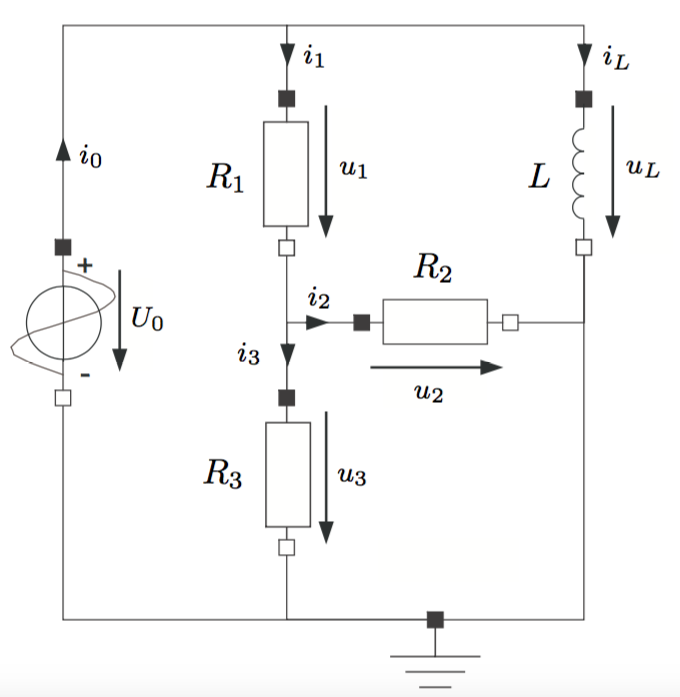
\includegraphics[width=0.8\textwidth]{graphics/rlc_loop.png}
        \end{column}
        \begin{column}{0.5\textwidth}
            \begin{eqnarray*}
            u_{0} & = & \sin\left(t\right)\\
            u_{1} & = & R_{1}i_{1}\\
            u_{2} & = & R_{2}i_{2}\\
            u_{L} & = & L\frac{di_{L}}{dt}\\
            i_{C} & = & C\frac{du_{C}}{dt}\\
            u_{0} & = & u_{1}+u_{2}\\
            u_{L} & = & u_{1}+u_{2}\\
            u_{C} & = & u_{2}\\
            i_{0} & = & i_{1}+i_{L}\\
            i_{1} & = & i_{2}+i_{C}
            \end{eqnarray*}
        \end{column}
    \end{columns}
\end{frame}
